\documentclass[../main.tex]{subfiles}

\begin{document}
\section{Discussion}

\subsection{Validation}
% Validation was good
Our behavioral experiment showed that GANalyze was indeed able to generate images of increasing aesthetic value as seen in the positive slope between the proportion agreement with the neural network and the $\alpha$-values. Even when forced to choose between two nearly identical images, our participants picked the image GANalyze generated to be more beautiful at rates above chance. The relation between GANalyze's $\alpha$-values and our participant's preference followed the shape of a typical psychometric curve in 2-AFC discrimination tasks, implying that the internal values of the neural network translate to human aesthetic appreciation similar to how for example auditory stimulus intensity translates to human auditory perception. Taken together, these findings hint towards the existence of objective properties of beauty which GANalyze has learned to manipulate. As we have confirmed that GANalyze is indeed able to manipulate these aesthetic qualities in images, we can now use these images to find what makes an image beautiful.


\subsection{Demographic Effects}
% Structural modeling interpretation
Through structural equation modeling, we have determined that while a shortened version of the AEQ is valid, the measured aesthetic experience does not influence the appraisal of image aesthetics in a behavioral experiment. Age and sex also have no effect on neither aesthetic experience, nor the aesthetic judgement in the experiment. Nationality on the other hand, may have a small effect on the aesthetic experience, which was not found in the original paper on the AEQ’s development by \textcite{wanzerExperiencingFlowViewing2020}. There was no effect of nationality on aesthetic judgement however. Taken together, these results seem to point towards the objective properties of beauty. However, because our analysis was on the group level, we can't make any claims on the effects of subjective variables. Furthermore, it is also possible that our aesthetic judgement outcome variable was not specific enough to detect the effects the latent aesthetic judgement may have had.

% Cross-cultural effects etc




\subsection{Behavioral Findings}
% Asymmetry
We found that while our participants were more likely to agree with the network for higher $\alpha$-values, their responses to high $\alpha$-values were different from those to low $\alpha$-values. To clarify this asymmetry: images that the network generated to be much less aesthetic than the neutral image were indeed rated much worse: at the most extreme value, namely $\alpha = -0.25$, our participants agreed with GANalyze $93\%$ of the time that the image with $\alpha = 0$ (i.e., the neutral image) was more beautiful than the image with $\alpha = -0.25$. From this we can conclude that GANalyze is very capable of making images \textit{less} aesthetic. When we look at the positive $\alpha$'s, we see a similar pattern. However, for the most extreme value, $\alpha = 0.25$, the agreement was at $81\%$. While we can still conclude that GANalyze is capable of making images more beautiful, the effects are less pronounced. 

It is not immediately clear whether this effect is caused by properties of human perception, or GANalyze's parameters. To investigate potential causes stemming from human perception, we will first illustrate a number of relevant theories from cognitive and biological psychology, after which we will situate our finding in the broader theoretical scope. Second, we will look into the possibility that it is the generated stimuli themselves that have caused this asymmetry.

\subsubsection{Perception-Based Explanation}
% Supernormal stimuli and peak shift principle
A supernormal stimulus in evolutionary and biological psychology is an exaggeration of a natural stimulus that evokes a stronger response than the natural one. We encounter these supernormal stimuli everywhere in daily life, from advertisements to propaganda \parencite{barrett2010supernormal}. It follows logically that applying stimuli such as these to art would evoke a stronger response. \textcite{costa2006aesthetic} found that people indeed have an aesthetic preference for exaggerated facial features such as roundness of eyes and lips. \textcite{ramachandran1999science} introduced a framework, the peak shift principle, in an attempt to `explain art'. The peak shift principle builds upon supernormal stimuli to claim that art is characterized by caricatures, referring to examples such as prehistoric cave paintings and the Venus `fertility' figures \parencite{ramachandran1999science}. In this framework, amplifying the distinguishing features of an object, even to the point of being completely unnatural, should result in higher aesthetic value. This is a controversial framework however, as it has been claimed to be made up of overly ambitious ideas, flawed argumentation, and unsubstantiated claims \parencite{hyman2010art}. While we have generally found an effect that seems to be in line with that framework in our study, the asymmetry of the positive and negative $\alpha$'s raises questions. 

% Relate findings to peak shift
From a peak shift perspective, it does not make sense that our participants show a decreased effect for the high-$\alpha$ images, as the framework would have predicted that the aesthetic reaction to the (perhaps unnaturally) exaggerated features of $\alpha=0.25$~images should be at least as strong as for $\alpha=-0.25$~images. The asymmetry we found then implies that there is likely more to it than \textcite{ramachandran1999science} had proposed. We argue that perceived realism also plays an important role in the aesthetic evaluation of images that are presented as a photograph. Taking realism into account, it makes sense that the most extreme negative $\alpha$'s are rated stronger compared to extreme positive $\alpha$'s. It is the images with extreme positive $\alpha$'s that may be perceived as simply `too much', or `artificial-looking'.

% Processing fluency
Approaching our findings from the perspective of the processing fluency theory \parencite{reberProcessingFluencyAesthetic2004} described in the introduction, this would imply that the images generated with the highest $\alpha$-values are processed at similar rates, regardless of the changing low-level features. Intuitively it makes sense that our low-level features initially boost processing fluency. At a certain point however, these objective changes may be overshadowed by subjective factors playing a relatively bigger role. These subjective factors are beyond the scope of this study however.


\subsubsection{GANalyze-Based Explanation}
It is also possible that the asymmetry was caused by the stimuli themselves rather than human perception. Inspecting the trajectories of the contrast and sharpness in Figure~\ref{fig:img_features}, shows that their effects slow down for the high positive $\alpha$-values. This could be the reason for these particular images not being rated much higher than those of adjacent lower $\alpha$-values. Why exactly GANalyze reduced the effects of contrast and sharpness is unclear. Perhaps the GAN had actually learned that unrealistic images with extreme image features are not appraised positively and therefore reduced the effects of contrasts and sharpness. But this hypothetical compensation seems not to have been very effective, as the extreme high $\alpha$-images are still rated lower than expected. Further research can potentially test this theory by grouping image sequences based on the intensities of contrast and sharpness of high-$\alpha$ images. This way, it could be possible to find out whether the compensatory moderation of contrast and sharpness indeed results in images of higher aesthetic quality. 

% High-level features
Another possible explanation comes from the influence of higher-level image features. Examples of such features are `harmony' and `balance', but also Gestalt principles such as figure-ground segmentation or the relative convexity and sharpness of the central object compared to the background. While these factors are not directly represented in any of the low-level features themselves, they may be disturbed by extremely high contrast and sharpness. It is possible that GANalyze has learned to prioritize these higher-level features over the low-level features separately. The increase in low-level features we observe in our results are then a consequence of GANalyze improving these higher-level features.


\subsection{A Visual Definition of Beauty}
Just as \textcite{goetschalckxGANalyzeVisualDefinitions2019} used GANalyze to make a visual definition of memorability, we made a visual definition of beauty. Our visual definition can be seen in Figure~\ref{img:visual_def}. We quantified the changes made to the images in four image features as suggested by \textcite{ke2006design}, shown in Figure~\ref{fig:img_features}. All of the image features we studied increased along with the $\alpha$-values. It would be naive however to claim that simply increasing the brightness, contrast, sharpness, and saturation of any given image would increase its aesthetic quality.

\begin{figure}[!ht]
	\caption{Visual Definition of Beauty}
	\label{img:visual_def}
	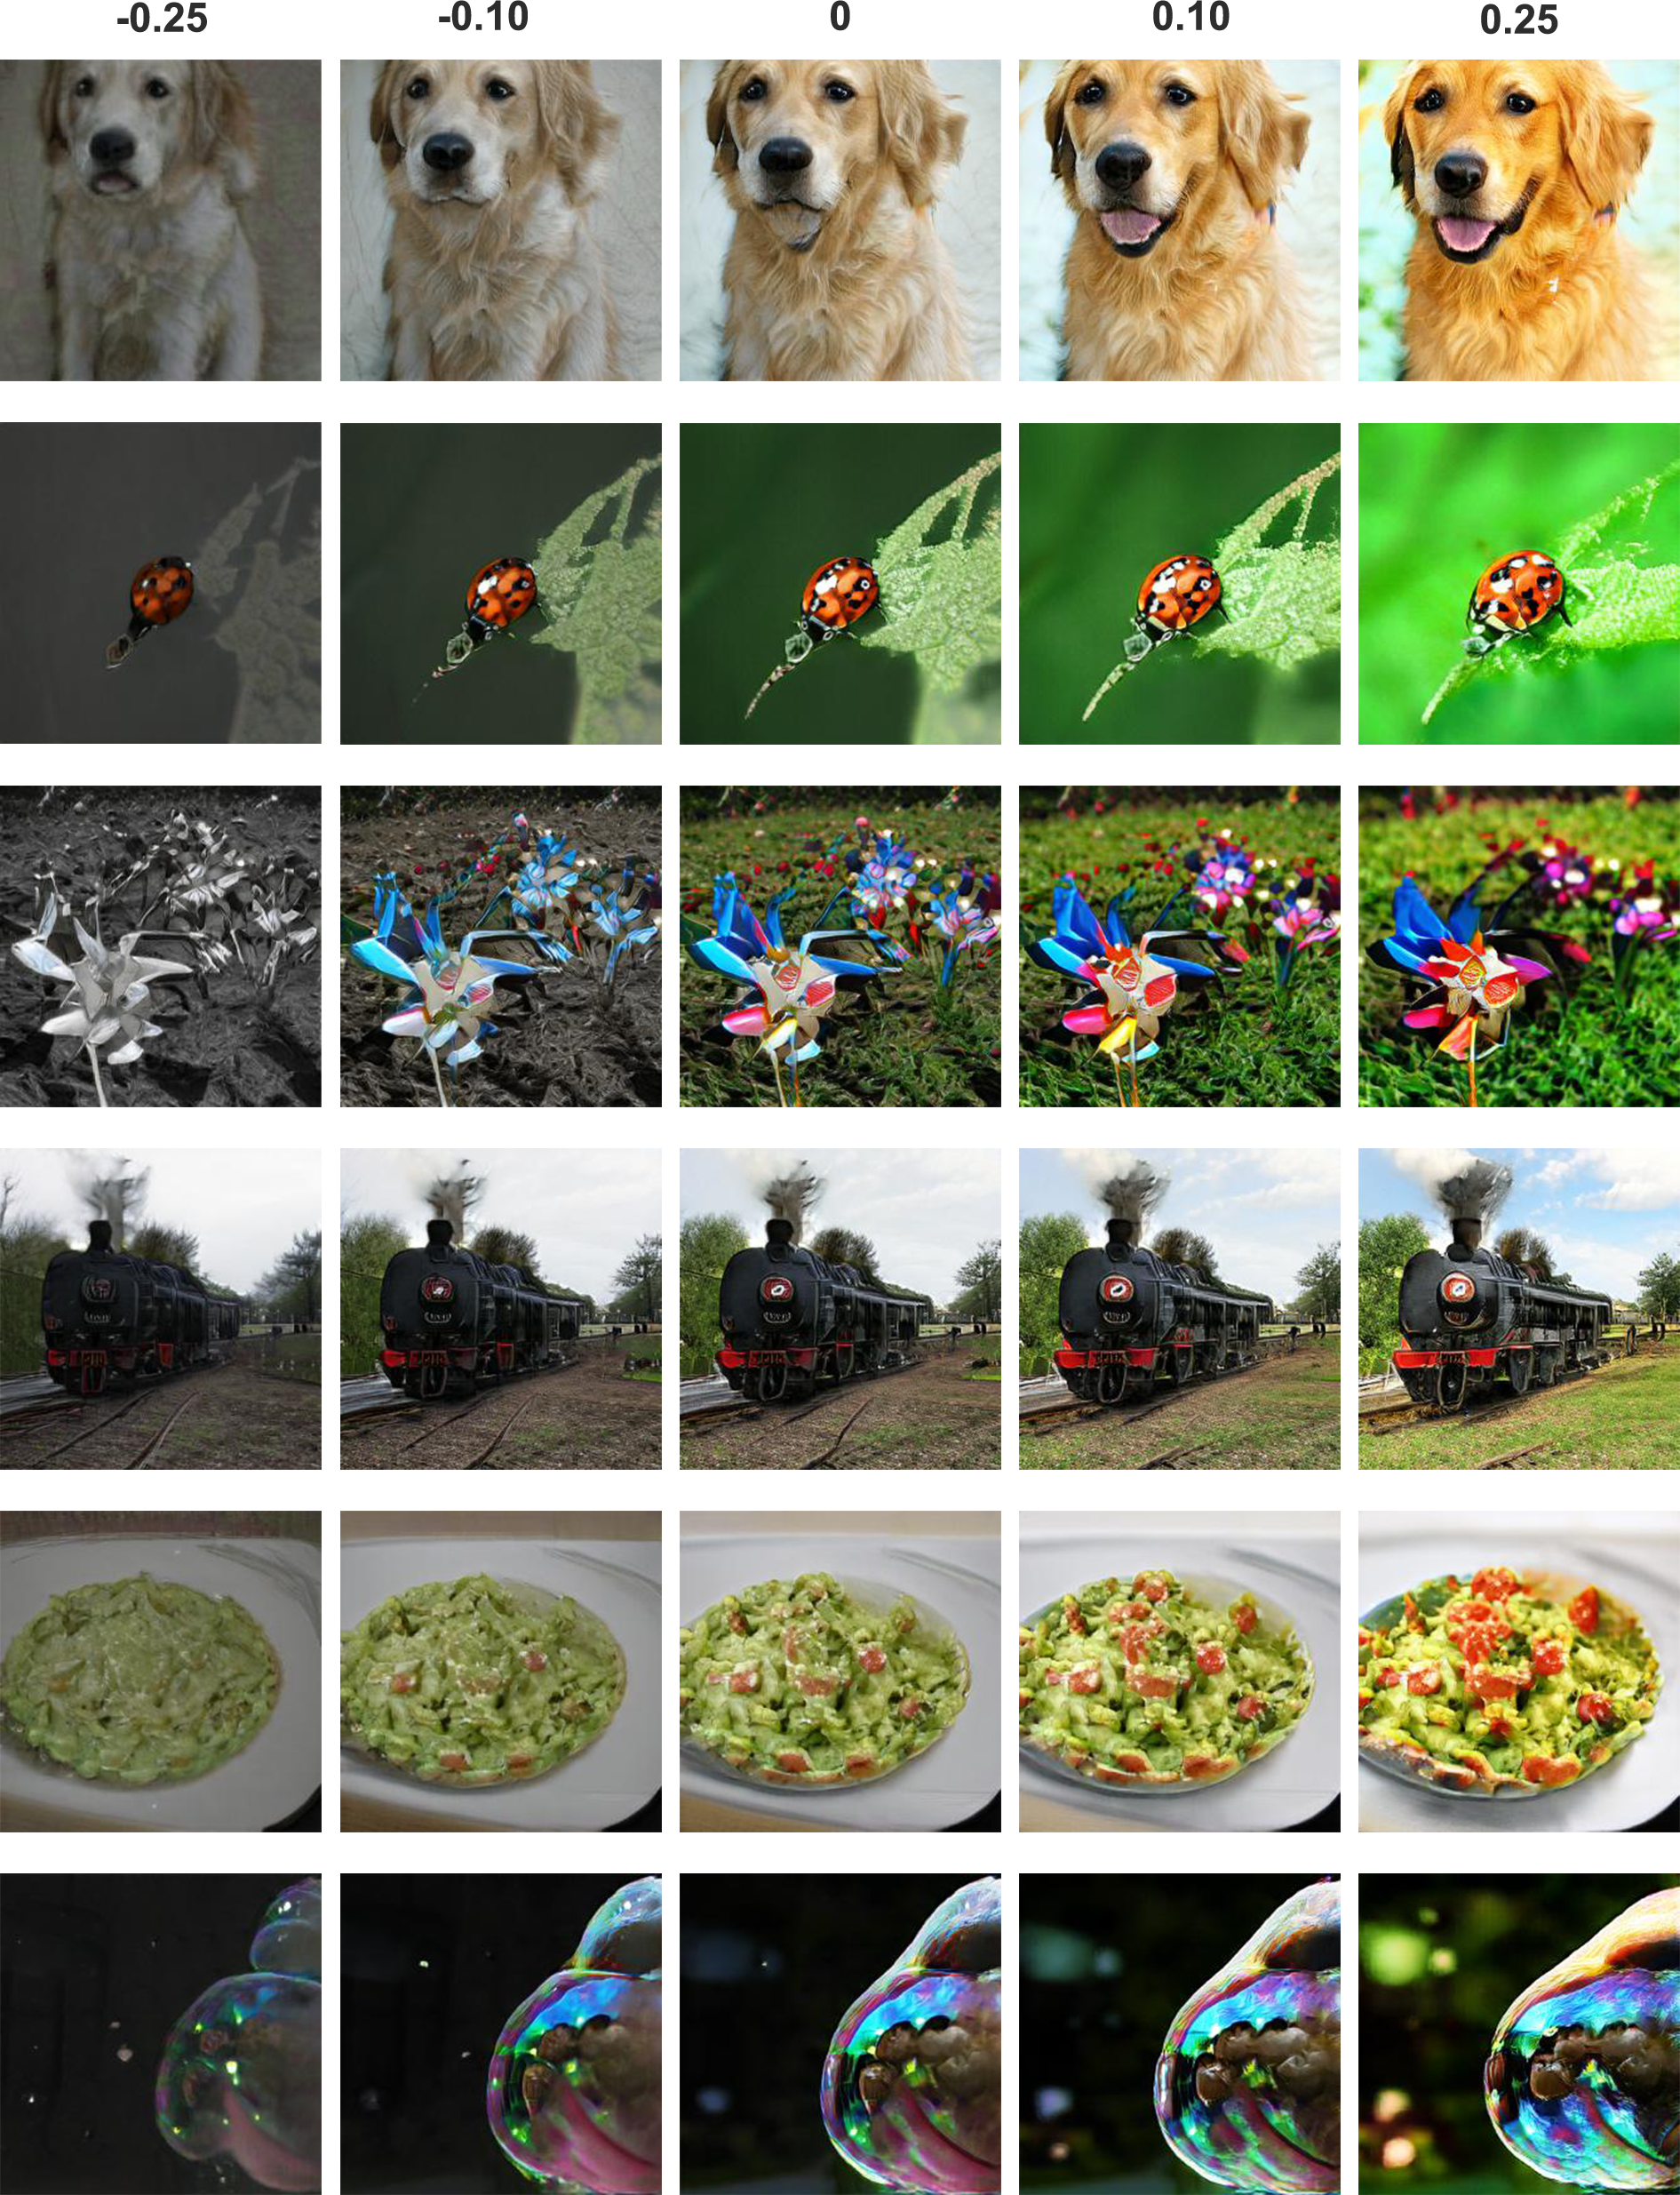
\includegraphics[width=1\linewidth]{images/visual_definition}
	{\textit{Note.} Our visual definition of beauty presented as the increasing aesthetic value of an image.}
\end{figure}

We have reasons to believe that instead of simply increasing these parameters, GANalyze instead used sophisticated methods acquired through deep learning to determine which features to modify, how intense the modification should be given a certain $\alpha$-value, and how the different image features interact with each other. For example, looking at the color distributions for five image sequences in Figure~\ref{fig:col_dists} shows that while there is indeed a pattern of moving towards the extremes of the spectrum, the way this happens differs between the image sequences. The most prominent colors tend to increase while the others decrease, but this differs for every image.

\subsubsection{Image Features}
\paragraph{Brightness.} The mean pixel values of grayscale images increased along with the $\alpha$-values, meaning that the images got brighter. While this is consistent with the literature, brightness in the context of aesthetics is often evaluated as relative brightness of the main object compared to the background \parencite{ke2006design, obrador2010role}, which we have not done in this study. A visual inspection of the image sequences does not seem to indicate specific changes to the relative brightness, as everything seems to increase. It is unclear if relative brightness is not as important as the literature makes it out to be, or GANalyze simply failed to implement it properly.

\paragraph{Contrast.} The spread of the grayscale pixels values grew, meaning that the contrast of the images increased. Contrast has also generally been found to correlate with aesthetic appraisal \parencite{wong2009saliency}, though they tend to differentiate between lightning contrast and color contrast, which we have not considered in the present study.

\paragraph{Sharpness.} The sharpness of images increased, which also a common finding \parencite{redi2015beauty}. Interestingly, for some images, GANalyze made the main subject sharper and added blur to the background, which is a more advanced transformation than simply making everything sharper. Sharpness in this sense contributes to the main subject of the image being featured more prominently, which is an important factor in aesthetic appraisal \parencite{wong2009saliency}.

\paragraph{Saturation.} Studies generally find that increasing the saturation of the main subject of an image is important for its aesthetics \parencite{wong2009saliency}. From a visual inspection however, GANalyze seems to increase the saturation for the image as a whole. However, because we did not measure the saturation of the main subject formally, we cannot confidently claim that GANalyze ignores this property.

\subsubsection{Visual Inspection}
Simply looking at the image sequences from our visual definition in Figure~\ref{img:visual_def} can give us some insight into the higher-level image features that change together with the $\alpha$-value. The first row for example shows the changes in low-level image features we previously discussed. However, a notable change from $\alpha=-0.25$ to $\alpha=0.25$ is the fact that the dog's emotional expression seems to change from sad or neutral, to happy with its tongue out. This is an example of a change that's impossible to quantify with only the low-level features we analyzed. It also demonstrates the potential capabilities GANs have for studying high-level cognitive properties. The fourth image sequence depicting a train shows a less pronounced effect. While the low-level image features do increase, the changes are not as obvious as in the other sequences. This image sequence also illustrates the decrease in realism that may have played a role in the asymmetry between positive and negative $\alpha$'s. The sixth image sequence, depicting a bowl of presumably guacamole, also shows an interesting effect on top of the low-level image features. As the $\alpha$ increases, more ingredients seem to appear.

While the patterns found in these visual inspections can be subjective, they do show that GANalyze, and as a consequence the aesthetic value of images, rely on more than just low-level image features. In other words, to make an image more beautiful, one has to do more than simply make them sharper and more colorful. The changes made to the higher-level features differ between each image, making it difficult to highlight the factors in question separately with our present resources.

\subsection{Limitations}
One limitation of our study is that it was limited to natural looking images being compared to a slightly different variation of themselves. Beauty and art are more than just a combination of low-level image features and colors. To address this limitation, future studies could use our stimuli to compare images from different image sequences to each other. As we have on average 20 ratings per individual image, it should be possible to compute the aesthetic value of each image and then compare images from different sequences with a similar score. This way, it may be possible to find more sophisticated features underlying the aesthetic value of these images, like for example image composition parameters such as the rule of thirds, or principles from Gestalt psychology.

Another limitation is that our experiment's design primarily relied on an objectivist conception of beauty. We did not pay much attention to individual differences in aesthetic appraisal other than broadly comparing the effects of demographic variables on the agreement with GANalyze. As it is believed that perception of beauty is an interaction between subjective and objective variables, it may prove beneficial to conduct a deeper investigation into the subjective part of the equation. For example, it may be possible to group images based on the most saliently changing low-level feature. The steepness of the psychometric functions may then be compared between individuals for each of the image features.


% Talk about the processing fluency theory mentioned in the introduction

\end{document}